\documentclass{article}
\usepackage[utf8]{inputenc}
\usepackage[T1]{fontenc}
\usepackage{booktabs}
\usepackage{graphicx}
\usepackage{hyperref}
\usepackage{xcolor}
\definecolor{validated}{HTML}{047857}
\definecolor{refuted}{HTML}{B91C1C}
\definecolor{inconclusive}{HTML}{9A3412}
\title{Empirical Proof Record: REFUTED}
\date{2026-05-15T13:04:36.612283+00:00}
\begin{document}
\maketitle
\section*{Empirical Proof Record --- \textcolor{refuted}{\textbf{REFUTED}}}
\textbf{Proof ID:} \texttt{19b0e547908eeaf788398f6ccdaab54a\dots}\\
\textbf{Created:} 2026-05-15T13:04:36.612283+00:00
\subsection*{1. Claim}
\begin{quote}On real technical-domain text (Linux kernel commit messages) that clears Kimera's GWF, the substrate's walker reaches sustained traversal (halt\_mode == 'exhausted') in >= 60\% of cycles — i.e. the topology layer engages on technical reasoning instead of collapsing to amplitude\_death.\end{quote}
\begin{itemize}
\item \textbf{Operationalisation:} fraction of GWF-cleared Linux-kernel-commit cycles for which result.halt\_mode == 'exhausted'
\item \textbf{Threshold:} \texttt{sustained\_traversal\_rate\_on\_cleared >= 0.6 fraction}
\item \textbf{H0:} P(halt='exhausted' | gwf cleared) < 0.6
\item \textbf{H1:} P(halt='exhausted' | gwf cleared) >= 0.6
\end{itemize}
\subsection*{2. Verdict}
\textcolor{refuted}{\textbf{REFUTED}} --- observed \texttt{0.39636913767019666}\\
walker reached sustained traversal in 262/661 GWF-cleared cycles (39.6\%); amplitude\_death in 191/661 (28.9\%); GWF blocked 339/1000 (33.9\%); halt modes observed: \{'exhausted': 262, 'selective': 208, 'amplitude\_death': 191\}; dissonance median=28 (range 0-49); Φ median=0.209; 1000 cycles, 0 adapter errors
\begin{figure}[h!]\centering
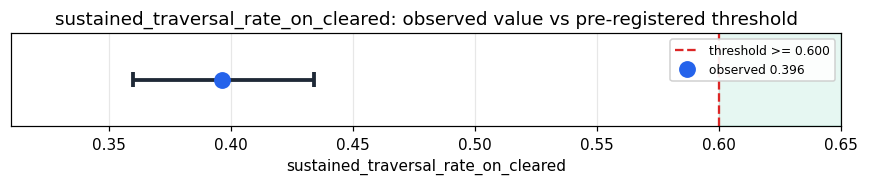
\includegraphics[width=0.8\linewidth]{assets/ci_sustained_traversal_rate_on_cleared}
\caption{sustained\_traversal\_rate\_on\_cleared -- observed value with Wilson 95\% CI.}
\end{figure}
\subsection*{3. Evidence}
\begin{tabular}{llrrl}\toprule
\textbf{Pillar} & \textbf{Statistic} & \textbf{Value} & \textbf{95\% CI} & \textbf{Library} \\\midrule
\texttt{O.topology.sustained\_traversal} & \texttt{sustained\_traversal\_rate\_on\_cleared} & \texttt{0.39636913767019666} & (0.3598, 0.4342) & statsmodels 0.14.6 \\
\texttt{O.topology.amplitude\_death\_rate} & \texttt{amplitude\_death\_rate\_on\_cleared} & \texttt{0.28895612708018154} & --- & ophamin 0.1.0 \\
\texttt{O.topology.halt\_mode\_distribution} & \texttt{halt\_modes\_observed\_count} & \texttt{3.0} & --- & ophamin 0.1.0 \\
\texttt{O.topology.gwf\_block\_rate} & \texttt{gwf\_block\_rate\_on\_linux} & \texttt{0.339} & --- & ophamin 0.1.0 \\
\texttt{O.topology.dissonance\_intensity} & \texttt{dissonance\_events\_count\_median} & \texttt{28.0} & --- & python-stdlib 3.14 \\
\texttt{O.topology.phi\_distribution} & \texttt{phi\_value\_median} & \texttt{0.20941038886785676} & --- & python-stdlib 3.14 \\
\bottomrule\end{tabular}
\subsection*{4. Pre-registration}
\begin{itemize}
\item Registered at: \texttt{2026-05-15T12:32:23.763443+00:00}
\item Config hash: \texttt{898ebda325a9dc57963638a7cf5ece8c\dots}
\item Data hash: \texttt{92a34cc4275008279006eeec2c19cd2b\dots}
\end{itemize}
\subsection*{5. Signature}
\texttt{5651b2e897f40c38607df311c27afecd0c96e5e5e710ab5e415c02c8e86b14f9}\\

\end{document}
